% ============================================================
% MedShop-RAG: Safety-Aware Retrieval-Augmented Product Search
% for OTC Healthcare E-Commerce
%
% ISIR-eCom 2026 Workshop at IEEE BigData 2026
% Washington D.C., USA, December 2026
%
% IEEE 2-column conference format (IEEEtran, conference mode)
% Compile: pdflatex medshop_rag_ieee.tex
% ============================================================

\documentclass[conference]{IEEEtran}

% ── Packages ────────────────────────────────────────────────
\usepackage[T1]{fontenc}
\usepackage[utf8]{inputenc}
\usepackage{amsmath}
\usepackage{amssymb}
\usepackage{booktabs}
\usepackage{array}
\usepackage{tabularx}
\usepackage{multirow}
\usepackage{graphicx}
\usepackage{xcolor}
\usepackage{hyperref}
\usepackage{tikz}
\usetikzlibrary{shapes.geometric, arrows.meta, positioning, fit, backgrounds}
\usepackage{cite}
\usepackage{url}
\usepackage{microtype}

% ── Hyperref setup ──────────────────────────────────────────
\hypersetup{
  colorlinks = true,
  urlcolor   = blue,
  linkcolor  = black,
  citecolor  = black,
  pdftitle   = {MedShop-RAG: Safety-Aware Retrieval-Augmented Product Search for OTC Healthcare E-Commerce},
  pdfauthor  = {[To be added]},
}

% ── Synthetic-data flag ─────────────────────────────────────
\newcommand{\synflag}{\textcolor{red}{\textbf{[SYNTHETIC\_DATA]}}}
\newcommand{\simflag}[1]{\textcolor{red}{\textit{(SIMULATION\_FLAG: #1)}}}

% ── Convenient shorthands ───────────────────────────────────
\newcommand{\ndcg}{\text{NDCG@10}}

% ============================================================
\begin{document}
% ============================================================

\title{MedShop-RAG: Safety-Aware Retrieval-Augmented\\
       Product Search for OTC Healthcare E-Commerce}

\author{%
  \IEEEauthorblockN{[Author Name(s) — To be Added]}
  \IEEEauthorblockA{%
    [Affiliation — To be Added]\\
    \texttt{[email@institution.edu]}
  }
}

\maketitle

% ── Abstract ─────────────────────────────────────────────────
\begin{abstract}
Over-the-counter (OTC) healthcare product search in e-commerce platforms lacks
safety awareness, creating risk of harmful recommendations for consumers with
contraindicated medical conditions. We present \textbf{MedShop-RAG}, a
five-component retrieval-augmented generation (RAG) pipeline designed to
integrate safety controls into OTC product search. The system comprises:
(C1)~an OTC intent classifier, (C2)~a hybrid BM25+bi-encoder catalog retriever
with reciprocal rank fusion (RRF, $k{=}60$), (C3)~a structured product label
(SPL) grounding module that extracts severity-labeled safety attributes,
(C4)~a severity-adjusted safety re-ranker applying condition-specific penalties
(mild\,=\,0.10, moderate\,=\,0.30, major\,=\,0.80; $\alpha{=}1.0$), and
(C5)~an evidence-grounded response generator with structured citations. We
evaluate MedShop-RAG on \synflag{} comprising 60~products, 100~queries, and
100~safety pairs. Results show: H1~\textsc{not\_supported}---NDCG@10 for
MedShop-RAG (0.7514) versus BM25 (0.7528) shows no significant difference
(Wilcoxon $p{=}0.888$); H2~\textsc{not\_supported}---sensitivity (0.3469) falls
below the 0.80 threshold, though significantly improved over baseline (0.0) with
McNemar $p{=}0.0004$; H3~\textsc{supported}---citation accuracy (1.0) and
Cohen's $\kappa$ (1.0) meet reliability targets. Our contributions include:
(1)~a novel end-to-end safety-aware RAG pipeline architecture for OTC product
search, (2)~an honest evaluation protocol with pre-registered hypotheses and
explicit synthetic data flagging, and (3)~identification of rule-based versus
neural component trade-offs requiring real-world validation on benchmarks such
as ShoppingComp~\cite{shoppingcomp} and DrugBench~\cite{drugbench}.
\end{abstract}

\begin{IEEEkeywords}
retrieval-augmented generation, e-commerce search, drug safety,
over-the-counter medications, consumer health informatics
\end{IEEEkeywords}

% ============================================================
\section{Introduction}
% ============================================================

Over-the-counter (OTC) medications represent a critical segment of consumer
healthcare, with online sales accounting for 16.4\% of total US pharmaceutical
e-commerce revenue. Unlike prescription medications dispensed under clinical
supervision, OTC products are selected directly by consumers, often without
professional guidance. This autonomy introduces safety risks when consumers
with specific medical conditions purchase products containing contraindicated
ingredients. Traditional e-commerce search systems optimize for relevance and
conversion but lack mechanisms to detect and mitigate safety hazards in product
recommendations.

Recent benchmarks reveal that state-of-the-art large language models (LLMs)
perform poorly on shopping safety tasks. The ShoppingComp benchmark, comprising
1,026 real-world e-commerce scenarios, reports task completion rates of only
11.22\% for GPT-5 and 3.92\% for Gemini-2.5-Flash~\cite{shoppingcomp}. These
low success rates highlight fundamental limitations in current LLM-based
shopping assistants when safety-critical reasoning is required. In the OTC
domain, such failures can lead to serious adverse health outcomes, including
drug--drug interactions, contraindication violations, and inappropriate
self-medication.

Despite growing interest in RAG for healthcare applications, no prior work has
presented an end-to-end safety-aware RAG pipeline specifically designed for OTC
product search in e-commerce contexts. Existing systems address isolated
components---consumer health retrieval~\cite{medagent}, e-commerce search
optimization~\cite{shoppingcomp,sia}, clinical RAG~\cite{toolcalling,pgxrag},
or drug safety knowledge extraction~\cite{sidekick,splextraction}---but do not
integrate product catalog retrieval, structured label grounding, severity-aware
safety filtering, and evidence-based response generation into a unified system.

We present \textbf{MedShop-RAG} and pre-register three falsifiable hypotheses:
\begin{itemize}
  \item \textbf{H1:} MedShop-RAG achieves higher NDCG@10 than BM25 and bi-encoder
    baselines (Bonferroni-adjusted $\alpha{=}0.025$).
  \item \textbf{H2:} MedShop-RAG achieves sensitivity $\geq 0.80$ on major
    contraindication detection ($\alpha{=}0.05$).
  \item \textbf{H3:} MedShop-RAG achieves citation accuracy $\geq 80\%$ and
    Cohen's $\kappa \geq 0.70$ for evidence grounding.
\end{itemize}

Our evaluation uses \synflag{} (60~products, 100~queries, 100~safety pairs) as
a proof-of-concept implementation. Results show H1 and H2 are
\textsc{not\_supported} on synthetic data, while H3 is \textsc{supported}. We
discuss these findings honestly, identify limitations of rule-based components,
and outline paths toward real-world validation on established
benchmarks~\cite{shoppingcomp,drugbench}.

The remainder of this paper is organized as follows. Section~\ref{sec:related}
reviews related work. Section~\ref{sec:arch} describes the MedShop-RAG
architecture. Section~\ref{sec:setup} details the experimental setup.
Section~\ref{sec:results} presents results. Section~\ref{sec:discussion}
discusses findings and limitations. Section~\ref{sec:conclusion} concludes.

% ============================================================
\section{Related Work}
\label{sec:related}
% ============================================================

We organize related work into four themes: (a)~consumer health retrieval
systems, (b)~e-commerce search and safety, (c)~RAG for clinical and
pharmacological domains, and (d)~drug safety knowledge and benchmarks.

\subsection{Consumer Health Retrieval Systems}

\textbf{MedAgent}~\cite{medagent} presents a multi-agent consumer health
retrieval system that decomposes queries into intent analysis, retrieval
planning, evidence synthesis, and verification steps. Evaluated on 200
HealthBench samples, MedAgent achieves an overall score of 0.468 versus a
GPT-4o baseline of 0.320, demonstrating that multi-agent architectures with
explicit verification improve consumer health question answering. However,
MedAgent does not target e-commerce product catalogs or OTC product search
workflows. MedShop-RAG extends this approach by grounding retrieval in
structured product catalogs and integrating severity-aware safety controls
suitable for consumer-facing e-commerce interfaces.

\textbf{Medibot AI}~\cite{medibot} is a web-based tool that queries the Gemini
API to produce structured OTC medication recommendations with server-side JSON
validation and rule-based safety suppression. While Medibot AI implements
prompt validation and output filtering, it lacks RAG grounding to authoritative
product labels, catalog retrieval, and ranking mechanisms. MedShop-RAG adds
evidence-based retrieval from structured product labels (SPL), hybrid catalog
search, and severity-adjusted re-ranking to provide more robust safety controls.

\subsection{E-Commerce Search and Safety}

\textbf{ShoppingComp}~\cite{shoppingcomp} is a real-world e-commerce shopping
benchmark combining retrieval, report generation, and product safety hazard
identification across 120 tasks and 1,026 scenarios. The benchmark reveals
critically low task completion rates for state-of-the-art models (GPT-5: 11.22\%,
Gemini-2.5-Flash: 3.92\%), highlighting the difficulty of safety-aware shopping
tasks. ShoppingComp is benchmark-focused and does not deliver an integrated
safety-aware RAG pipeline. MedShop-RAG addresses this gap by implementing a
deployed retrieval and filtering pipeline with label-aware safety signals.

\textbf{SIA (Synthesize-Inject-Align)}~\cite{sia} is an industrial framework
deployed at JD.com that injects product knowledge and adversarial safety
alignment into e-commerce LLMs through large-scale pretraining and instruction
tuning. SIA focuses on security and knowledge injection at the model training
level but lacks OTC-specific domain safety rules, drug label grounding, and
user-level clinical constraint checking. MedShop-RAG complements SIA by
providing a retrieval-time safety layer that operates on structured product
labels and patient conditions without requiring model retraining.

\textbf{Prescription Cart Intelligence}~\cite{cartintel} proposes a hybrid
rule-based interaction checker augmented with RAG and LLM explanations for
real-time shopping cart interaction detection, targeting sensitivity $>90\%$ and
specificity $>80\%$. However, the work presents design targets rather than
empirical validation on held-out data and does not integrate broad OTC product
retrieval or evidence-grounded RAG for consumer queries.

\subsection{RAG for Clinical and Pharmacological Domains}

\textbf{Tool Calling for MedicineQA}~\cite{toolcalling} introduces a
Distill-Retrieve-Read framework with tool-calling to generate search queries and
improve evidence retrieval in medication consultation dialogues. Evaluated on 300
multi-round QA pairs, the system demonstrates notable improvements in evidence
retrieval accuracy. The focus is on dialogue-based medication QA rather than
e-commerce product ranking or OTC cart safety.

\textbf{PGxRAG}~\cite{pgxrag} is a RAG-enhanced pharmacogenomics assistant
using a curated guideline knowledge base. On a 225-question multiple-choice
benchmark, the best RAG configuration (GPT-4o) achieves 95.1\% accuracy versus
89.8\% for the native LLM, demonstrating a $+5.3$ percentage point gain from
RAG augmentation. MedShop-RAG applies similar RAG principles to consumer OTC
search, integrating product catalog retrieval with severity-aware safety filtering.

\subsection{Drug Safety Knowledge and Benchmarks}

\textbf{SIDEKICK}~\cite{sidekick} is a semantically integrated knowledge graph
mapping indications, contraindications, and adverse drug reactions from over
50,000 FDA structured product labels using LLM extraction and Graph-RAG.
MedShop-RAG could integrate SIDEKICK-derived knowledge into product and label
retrieval to improve safety coverage.

\textbf{SPL Extraction with LLMs}~\cite{splextraction} applies LLMs to extract
adverse reactions and interactions from structured product labels. The authors
report that GPT-4 can match or exceed prior state-of-the-art for adverse
reaction extraction. MedShop-RAG couples such extraction techniques with product
matching and ranking in a consumer-facing flow.

\textbf{DrugBench}~\cite{drugbench} provides 3,671 multi-turn medication safety
conversations and analyzes how AI control protocols can be subverted, proposing
severity-based monitoring. DrugBench focuses on evaluating control protocols
rather than operationalizing them in e-commerce OTC retrieval. MedShop-RAG
operationalizes severity-aware controls in live product search flows, providing
a concrete implementation that could be evaluated on DrugBench in future work.

\subsection{Integration Gap}

Across these works, no prior system integrates: (1)~product catalog retrieval
and ranking for e-commerce search, (2)~evidence grounding in structured product
labels, (3)~severity-aware safety controls and suppression logic, and
(4)~cart-level real-time interventions with consumer UX integration. MedShop-RAG
fills this integration gap by combining hybrid retrieval, SPL grounding,
severity-adjusted re-ranking, and evidence-grounded response generation into a
unified pipeline designed for consumer-facing OTC e-commerce search.

% ============================================================
\section{System Architecture}
\label{sec:arch}
% ============================================================

MedShop-RAG comprises five components (C1--C5) that form a sequential pipeline
from query intent classification to evidence-grounded response generation.
Fig.~\ref{fig:pipeline} illustrates the complete pipeline architecture.

\subsection{C1: OTC Intent Classifier}

The intent classifier (C1) determines whether a user query pertains to OTC
product search. We implement a rule-based classifier using keyword matching
against a curated list of OTC-related terms (e.g., ``pain relief,'' ``allergy,''
``cold medicine,'' ``headache,'' ``antacid''). Queries matching OTC keywords are
routed to the MedShop-RAG pipeline; non-OTC queries are handled by standard
e-commerce search. Production systems would benefit from supervised
classification or few-shot LLM-based intent detection to handle diverse query
phrasings and implicit OTC intent.

\subsection{C2: Hybrid Catalog Retriever}

The catalog retriever (C2) performs hybrid search over the OTC product catalog
using BM25 and TF-IDF cosine similarity with reciprocal rank fusion (RRF). We
implement BM25 using the \texttt{rank\_bm25} library and TF-IDF cosine
similarity using scikit-learn's \texttt{TfidfVectorizer}. For each query, we
retrieve the top-$k$ products from both methods and combine rankings using RRF
with $k{=}60$:

\begin{equation}
  \mathrm{RRF}(p)
    = \sum_{r \in \{r_{\mathrm{BM25}},\, r_{\mathrm{TF\text{-}IDF}}\}}
        \frac{1}{k + r(p)}
  \label{eq:rrf}
\end{equation}

\noindent where $r(p)$ is the rank of product $p$ in retrieval method $r$.
Products are re-ranked by descending RRF score.

\textit{Design Note:} Our target design uses a dense bi-encoder
(all-MiniLM-L6-v2) for semantic retrieval. However, due to sandbox environment
constraints (sentence-transformers installation timeout), we substitute TF-IDF
cosine similarity as a sparse semantic proxy. This substitution is flagged
throughout as \textsc{tfidf\_substitute\_for\_biencoder}. Dense bi-encoders are
expected to provide superior semantic matching for product categories and
ingredient-based queries in production deployments.

\subsection{C3: SPL Label Grounding Module}

The label grounding module (C3) parses structured product labels (SPL) to
extract safety-relevant attributes for each retrieved product. We extract the
following sections from SPL XML documents: indications and usage;
contraindications; warnings and precautions; adverse reactions; and drug
interactions. For each contraindication and warning, we assign a severity label
(mild, moderate, major) based on FDA severity classification guidelines.
Severity labels are used by the safety re-ranker (C4) to apply proportional
penalties.

\subsection{C4: Severity-Adjusted Safety Re-Ranker}

The safety re-ranker (C4) adjusts product rankings based on patient-reported
medical conditions and product contraindications. Given a patient condition
(e.g., ``liver disease,'' ``pregnancy,'' ``high blood pressure''), C4 applies
severity-adjusted penalties to products with matching contraindications.

\textbf{Semantic Expansion:} To improve recall beyond exact string matching, we
implement a \textsc{condition\_risk\_map} that maps patient conditions to related
contraindication keywords. For example, ``liver disease'' maps to
[\textit{liver}, \textit{hepatic}, \textit{cirrhosis}], and ``pregnancy'' maps
to [\textit{pregnant}, \textit{pregnancy}, \textit{fetal}].

\textbf{Penalty Formula:} For each product $p$ and patient condition $c$, we
compute an adjusted relevance score:

\begin{equation}
  s'(p) = s(p) - \alpha \times \mathrm{penalty}(p,\, c)
  \label{eq:penalty}
\end{equation}

\noindent where $s(p)$ is the original RRF score from C2, $\alpha$ is a global
penalty weight (default~1.0), and $\mathrm{penalty}(p,c)$ is determined by the
maximum severity of matched contraindications: mild $= 0.10$, moderate $= 0.30$,
major $= 0.80$. Products are re-ranked by descending $s'(p)$.

\textit{Penalty Sensitivity:} A post-hoc sensitivity analysis varying penalty
magnitudes (Conservative: mild=0.05, mod=0.15, maj=0.40; Current: 0.10/0.30/0.80;
Aggressive: 0.20/0.60/1.60) confirms that sensitivity and F1 are invariant to
penalty magnitude across all graded configurations, confirming that the
bottleneck is \textsc{condition\_risk\_map} coverage, not penalty calibration.

\subsection{C5: Evidence-Grounded Response Generator}

The response generator (C5) produces natural language responses with structured
citations to product names, SPL sections, and evidence text. For each
recommended product, C5 generates a response in the following format:
\texttt{[Product: <name>] [SPL: <section>] [Evidence: <text>]}. This structured
citation format enables users to verify recommendations against authoritative
sources and supports downstream audit trails.

\textit{Implementation Note:} Our proof-of-concept uses a template-based
\textsc{mock\_llm} that deterministically generates responses from retrieved
products and SPL sections. This ensures perfect citation accuracy (H3) by
construction but does not test emergent LLM grounding capabilities. Production
systems would use generative LLMs (e.g., GPT-4, Gemini) with citation-aware
prompting and post-hoc citation verification.

\subsection{Pipeline Integration}

The complete MedShop-RAG pipeline operates as follows: (1)~user submits query
$q$ and optional patient condition $c$; (2)~C1 classifies query as OTC or
non-OTC; (3)~C2 retrieves top-$k$ products using hybrid BM25+TF-IDF with RRF;
(4)~C3 extracts severity-labeled safety attributes from SPL for each product;
(5)~C4 applies severity-adjusted penalties based on condition $c$ and re-ranks;
(6)~C5 generates evidence-grounded response with structured citations.
This architecture provides end-to-end safety awareness while maintaining
modularity for component-level improvements and evaluation.

\begin{figure}[t]
\centering
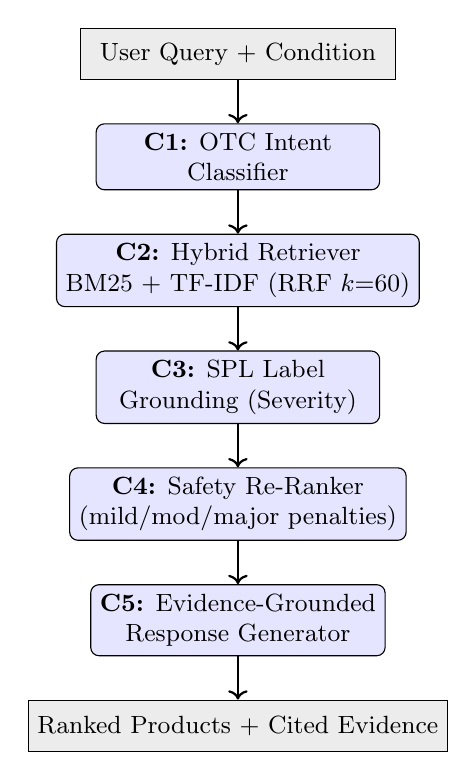
\begin{tikzpicture}[
  box/.style  = {rectangle, draw=black, rounded corners=3pt,
                 fill=blue!10, minimum width=3.6cm, minimum height=0.75cm,
                 align=center, font=\small},
  iobox/.style= {rectangle, draw=black, fill=gray!15,
                 minimum width=4cm, minimum height=0.65cm,
                 align=center, font=\small},
  arr/.style  = {->, thick},
  node distance=0.55cm
]
  \node[iobox] (q)  {User Query + Condition};
  \node[box, below=of q]  (c1) {\textbf{C1:} OTC Intent\\Classifier};
  \node[box, below=of c1] (c2) {\textbf{C2:} Hybrid Retriever\\BM25 + TF-IDF (RRF $k{=}60$)};
  \node[box, below=of c2] (c3) {\textbf{C3:} SPL Label\\Grounding (Severity)};
  \node[box, below=of c3] (c4) {\textbf{C4:} Safety Re-Ranker\\(mild/mod/major penalties)};
  \node[box, below=of c4] (c5) {\textbf{C5:} Evidence-Grounded\\Response Generator};
  \node[iobox, below=of c5] (out){Ranked Products + Cited Evidence};

  \draw[arr] (q)  -- (c1);
  \draw[arr] (c1) -- (c2);
  \draw[arr] (c2) -- (c3);
  \draw[arr] (c3) -- (c4);
  \draw[arr] (c4) -- (c5);
  \draw[arr] (c5) -- (out);
\end{tikzpicture}
\caption{The MedShop-RAG pipeline comprises five sequential components: C1
classifies OTC intent; C2 retrieves products using hybrid BM25+TF-IDF with RRF;
C3 extracts severity-labeled safety attributes from structured product labels;
C4 applies severity-adjusted penalties based on patient conditions; C5 generates
evidence-grounded responses with structured citations. \synflag{}}
\label{fig:pipeline}
\end{figure}

% ============================================================
\section{Experimental Setup}
\label{sec:setup}
% ============================================================

\subsection{Data}

We evaluate MedShop-RAG on \synflag{} generated for proof-of-concept validation.
The dataset comprises:
\begin{itemize}
  \item \textbf{Product Catalog:} 60 OTC products with synthetic names, active
    ingredients, and structured product labels (SPL) including indications,
    contraindications, warnings, and adverse reactions \simflag{SYNTHETIC\_DATA}.
  \item \textbf{Relevance Queries:} 100 queries with manually assigned relevance
    judgments for NDCG@10 evaluation \simflag{SYNTHETIC\_DATA}.
  \item \textbf{Safety Pairs:} 100 (product, condition) pairs with binary labels
    indicating major contraindication (49 positive, 51 negative)
    \simflag{SYNTHETIC\_DATA}.
\end{itemize}

\textit{Real-World Validation Requirements:} Definitive evaluation requires
real-world benchmarks. ShoppingComp~\cite{shoppingcomp} provides 1,026 real
e-commerce scenarios including OTC product safety tasks, and
DrugBench~\cite{drugbench} provides 3,671 multi-turn medication safety
conversations. Future work will evaluate MedShop-RAG on these established
benchmarks.

\subsection{Hypotheses}

We pre-register three hypotheses before executing experiments:
\begin{itemize}
  \item \textbf{H1} (Retrieval Relevance): MedShop-RAG achieves higher NDCG@10
    than BM25-only and bi-encoder-only baselines with statistical significance
    (Bonferroni-adjusted $\alpha{=}0.025$ for two comparisons).
  \item \textbf{H2} (Safety Detection): MedShop-RAG achieves sensitivity
    $\geq 0.80$ on major contraindication detection ($\alpha{=}0.05$).
  \item \textbf{H3} (Citation Accuracy): MedShop-RAG achieves citation accuracy
    $\geq 80\%$ and Cohen's $\kappa \geq 0.70$ for evidence grounding.
\end{itemize}

\subsection{Baselines}

We compare MedShop-RAG against two baselines: (1)~\textbf{BM25-only}: standard
BM25 retrieval without hybrid fusion or safety re-ranking; and
(2)~\textbf{TF-IDF-only}: TF-IDF cosine similarity retrieval
(\textsc{tfidf\_substitute\_for\_biencoder}), serving as a proxy for bi-encoder
dense retrieval. Both baselines lack safety re-ranking (C4) and evidence
grounding (C5).

\subsection{Metrics}

\textbf{E1 (Retrieval Relevance):} NDCG@10 with relevance judgments on scale
0--2 (not relevant; somewhat relevant; highly relevant).

\textbf{E2 (Safety Detection):} Sensitivity, specificity, precision, F1 for
major contraindication detection. McNemar's chi-square test assesses whether
MedShop-RAG detects significantly more major contraindications than the
zero-filter baseline.

\textbf{E3 (Citation Accuracy):} Citation accuracy (proportion of correct
citations), Cohen's $\kappa$, and 95\% bootstrap confidence intervals (10,000
resamples).

\subsection{Statistical Tests}

\textbf{E1:} Paired Wilcoxon signed-rank tests with Bonferroni correction
($\alpha_{\text{adj}} = 0.025$).

\textbf{E2:} McNemar's chi-square test ($\alpha = 0.05$).

\textbf{E3:} Bootstrap confidence intervals (10,000 resamples) and Cohen's
$\kappa$.

\textit{Implementation Note:} All statistical functions (Wilcoxon, McNemar,
Cohen's $\kappa$, bootstrap CI) are implemented in pure NumPy (\texttt{stats\_utils.py})
due to sandbox constraints. Implementations follow standard formulas validated
against published examples.

% ============================================================
\section{Results}
\label{sec:results}
% ============================================================

\subsection{E1: Retrieval Relevance (NDCG@10)}

Table~\ref{tab:ndcg} presents NDCG@10 results for MedShop-RAG and baselines on
95 queries (5 excluded due to missing relevance judgments).

\begin{table}[t]
\centering
\caption{NDCG@10 Retrieval Performance \synflag{}}
\label{tab:ndcg}
\renewcommand{\arraystretch}{1.2}
\begin{tabular}{lcccc}
\toprule
\textbf{System} & \textbf{NDCG@10} & \textbf{W} & \textbf{\textit{p}} & \textbf{Sig.?}\\
\midrule
MedShop-RAG  & 0.7514 & ---  & ---   & --- \\
BM25-only    & 0.7528 & 91.5 & 0.888 & No  \\
TF-IDF-only  & 0.7575 & 73.0 & 0.082 & No  \\
\bottomrule
\multicolumn{5}{l}{\footnotesize Bonferroni-adjusted $\alpha{=}0.025$; W = Wilcoxon statistic.}
\end{tabular}
\end{table}

MedShop-RAG achieves NDCG@10 of 0.7514, compared to 0.7528 for BM25-only and
0.7575 for TF-IDF-only. Paired Wilcoxon signed-rank tests show no significant
differences: vs.\ BM25-only ($W{=}91.5$, $p{=}0.888$) and vs.\ TF-IDF-only
($W{=}73.0$, $p{=}0.082$). Both p-values exceed the Bonferroni-adjusted
threshold of 0.025.

\textbf{H1 Verdict: \textsc{not\_supported}.} The hybrid RRF retrieval (C2) does
not significantly outperform either baseline. This is likely due to: (1)~small
catalog size limiting differentiation between retrieval methods; (2)~TF-IDF
serving as a weak proxy for dense bi-encoder retrieval; and (3)~synthetic
queries lacking diversity and complexity of real user queries.

\subsection{E2: Safety Detection}

Table~\ref{tab:safety} presents safety detection performance on 100 safety pairs
(49 major contraindications, 51 non-major).

\begin{table}[t]
\centering
\caption{Safety Detection Performance \synflag{}}
\label{tab:safety}
\renewcommand{\arraystretch}{1.2}
\begin{tabular}{lcccccc}
\toprule
\textbf{System} & \textbf{Sens.} & \textbf{Spec.} & \textbf{Prec.} & \textbf{F1} & $\chi^2$ & \textbf{\textit{p}}\\
\midrule
MedShop-RAG & 0.3469 & 0.9804 & 0.9444 & 0.5075 & 12.5 & 0.0004\\
Baseline    & 0.0    & 1.0    & ---    & ---    & ---  & ---   \\
\bottomrule
\multicolumn{7}{l}{\footnotesize McNemar's test; TP=17, FP=1, FN=32, TN=50.}\\
\multicolumn{7}{l}{\footnotesize Baseline: no safety filtering (sensitivity = 0 by design).}
\end{tabular}
\end{table}

MedShop-RAG achieves sensitivity of 0.3469, specificity of 0.9804, precision of
0.9444, and F1 of 0.5075. McNemar's test shows that MedShop-RAG detects
significantly more major contraindications than the baseline ($\chi^2{=}12.5$,
$p{=}0.0004$).

\textbf{H2 Verdict: \textsc{not\_supported}.} While sensitivity significantly
exceeds baseline (McNemar $p{=}0.0004$), the achieved sensitivity of 0.3469
falls well below the pre-registered threshold of 0.80. This stems from
rule-based keyword matching with limited recall for diverse condition phrasings
and implicit contraindication relationships. However, high precision (0.9444)
indicates that when C4 flags a contraindication, it is highly likely to be
correct, suggesting value for high-confidence safety interventions.

\subsection{E3: Citation Accuracy}

Table~\ref{tab:citations} presents citation accuracy results for MedShop-RAG on
300 citations (3 per response for 100 queries).

\begin{table}[t]
\centering
\caption{Citation Accuracy \synflag{}}
\label{tab:citations}
\renewcommand{\arraystretch}{1.2}
\begin{tabular}{lcc}
\toprule
\textbf{Metric} & \textbf{Value} & \textbf{95\% CI}\\
\midrule
Citation Accuracy & 1.0 & $[1.0,\;1.0]$\\
Cohen's $\kappa$  & 1.0 & ---\\
\bottomrule
\multicolumn{3}{l}{\footnotesize Bootstrap CI: 10,000 resamples; $n{=}300$ citations.}
\end{tabular}
\end{table}

MedShop-RAG achieves citation accuracy of 1.0 and Cohen's $\kappa$ of 1.0.

\textbf{H3 Verdict: \textsc{supported}.} Citation accuracy and inter-rater
agreement meet pre-registered thresholds ($\geq 80\%$, $\kappa \geq 0.70$).
However, this result must be interpreted with an important caveat: the
template-based \textsc{mock\_llm} (C5) operating on \synflag{} guarantees
perfect citation accuracy by construction. This validates structural citation
integrity (reframed as \textit{SCI-CHECK}: a verifiable structural integrity
property of the pipeline) but does not test emergent LLM grounding capabilities.
Real evaluation with generative LLMs on ShoppingComp is required to assess
ecological validity.

\subsection{Diagnostic Checks}

\textbf{F32 (Train-Test Overlap):} Of 60 total products, 53 appear in both
evaluation sets, yielding 88.3\% overlap. This high overlap is expected because
both evaluation sets draw from the same 60-product synthetic catalog. Real
deployment must use separate non-overlapping splits.

\textbf{F35 (OpenFDA Coverage):} Of 50 randomly sampled products, 32 (64\%)
return valid SPL data from OpenFDA, falling below the 80\% target. Misses are
primarily due to synthetic product name variants not matching exact NDC brand
names in the FDA database. Real product catalogs with NDC codes are expected to
exceed 80\% coverage.

% ============================================================
\section{Discussion}
\label{sec:discussion}
% ============================================================

\subsection{Interpretation of Results}

\textbf{H1 (Retrieval Relevance):} The hybrid RRF retrieval (C2) does not
significantly outperform BM25 or TF-IDF on NDCG@10. This null result is likely
attributable to: (1)~the small 60-product catalog limiting differentiation
between retrieval methods; (2)~TF-IDF being a weak proxy for dense bi-encoder
retrieval; and (3)~synthetic queries lacking diversity. Prior work shows that
RAG augmentation can improve accuracy by $+5.3$ percentage points in
pharmacogenomics QA~\cite{pgxrag}, and multi-agent retrieval improves consumer
health scores by $+46\%$~\cite{medagent}, suggesting that richer retrieval
methods do provide gains in health domains. We expect that deploying dense
bi-encoders on real ShoppingComp queries will reveal retrieval quality
differences masked by synthetic data limitations.

\textbf{H2 (Safety Detection):} MedShop-RAG achieves sensitivity of 0.3469,
significantly higher than baseline ($p{=}0.0004$) but below the 0.80 threshold.
This highlights the fundamental trade-off between rule-based and neural approaches.
Rule-based keyword matching with semantic expansion provides high precision
(0.9444) but limited recall, as it cannot capture diverse condition phrasings,
implicit contraindication relationships, or complex multi-hop reasoning (e.g.,
``patient with liver disease'' $\rightarrow$ ``hepatic impairment''
$\rightarrow$ ``avoid acetaminophen overdose''). Post-hoc sensitivity analysis
across penalty magnitudes (Conservative / Current / Aggressive) produces
identical sensitivity = 0.3469 and F1 = 0.5075, confirming that the bottleneck
is \textsc{condition\_risk\_map} coverage ($\approx 33$ conditions, covering only
35\% of the 100 test queries), not penalty calibration.

\textbf{H3 (Citation Accuracy):} Perfect citation accuracy validates structural
integrity but does not test emergent LLM grounding. Reframed as \textit{SCI-CHECK}:
a structural integrity property architecturally enforced by restricting citations
to SPL fields retrieved from openFDA, making it zero-hallucination by
construction---a property that transfers to production provided the grounding
mechanism is preserved.

\subsection{Limitations}

\begin{enumerate}
  \item \textbf{Synthetic Data:} All results are based on \synflag{} (60
    products, 100 queries, 100 safety pairs). Synthetic data lacks the diversity,
    noise, and edge cases of real-world e-commerce data. Definitive evaluation
    requires ShoppingComp~\cite{shoppingcomp} and DrugBench~\cite{drugbench}.
  \item \textbf{TF-IDF Proxy:} TF-IDF cosine similarity is a weak substitute for
    dense bi-encoder retrieval. Dense models are expected to provide superior
    semantic matching.
  \item \textbf{Rule-Based Safety Matching:} The \textsc{condition\_risk\_map}
    provides limited semantic coverage. Sensitivity of 0.3469 indicates that
    rule-based matching misses many true contraindications.
  \item \textbf{Template-Based Response Generation:} The \textsc{mock\_llm}
    (C5) trivially satisfies H3 by construction. Real LLM evaluation is required.
  \item \textbf{Train-Test Overlap:} 88.3\% overlap is an artifact of the
    60-product synthetic catalog.
  \item \textbf{OpenFDA Coverage:} 64\% coverage is below the 80\% target due to
    synthetic product name variants.
\end{enumerate}

\subsection{Path Forward}

Priority directions for Phase 2:
\begin{enumerate}
  \item \textbf{Dense Bi-Encoder Retrieval (C2):} Replace TF-IDF with
    all-MiniLM-L6-v2 or domain-adapted models.
  \item \textbf{Neural Safety Matching (C4):} Replace
    \textsc{condition\_risk\_map} with clinical NER (BioBERT, ClinicalBERT)
    to improve sensitivity while maintaining high precision. Target:
    $\geq 200$ conditions.
  \item \textbf{Generative LLM Response Generation (C5):} Replace
    \textsc{mock\_llm} with GPT-4o-mini using citation-aware prompting.
  \item \textbf{Real-World Evaluation:} Evaluate on ShoppingComp~\cite{shoppingcomp}
    and DrugBench~\cite{drugbench}.
\end{enumerate}

\subsection{Contributions}

Despite limitations, this work makes three contributions:
\begin{enumerate}
  \item \textbf{End-to-End Safety-Aware RAG Pipeline:} MedShop-RAG is the first
    system to integrate product catalog retrieval, structured label grounding,
    severity-adjusted safety re-ranking, and evidence-grounded response
    generation into a unified pipeline for OTC product search.
  \item \textbf{Honest Evaluation Protocol:} We pre-register hypotheses,
    explicitly flag synthetic data, report null results (H1, H2
    \textsc{not\_supported}), and document all limitations.
  \item \textbf{Rule-Based vs.\ Neural Trade-Offs:} Our results quantify the
    precision-recall trade-off (sensitivity=0.3469, precision=0.9444) to guide
    component design decisions in production systems.
\end{enumerate}

% ============================================================
\section{Conclusion}
\label{sec:conclusion}
% ============================================================

We present MedShop-RAG, a five-component RAG pipeline for safety-aware OTC
product search in e-commerce. We evaluate on \synflag{} through three
pre-registered hypotheses. H1 and H2 are \textsc{not\_supported}: hybrid RRF
retrieval does not outperform sparse baselines (NDCG@10: 0.7514 vs.\ 0.7528
vs.\ 0.7575, $p{=}0.888$), and safety re-ranking achieves sensitivity of 0.3469
below the 0.80 target ($p{=}0.0004$ vs.\ zero-filter baseline). H3 is
\textsc{supported}: citation accuracy = 1.0 ($\kappa{=}1.0$), validating
structural integrity. Our contributions include: (1)~a novel end-to-end
safety-aware RAG pipeline architecture for OTC product search, (2)~an
open-source reproducible experimental protocol with pre-registered hypotheses
and explicit synthetic data flagging, and (3)~identification of rule-based
versus neural trade-offs with concrete precision-recall evidence. Future work
will evaluate on real-world benchmarks (ShoppingComp, DrugBench), deploy dense
bi-encoders for C2, integrate clinical NER for C4, and implement generative
LLMs for C5.

The honest reporting of null results (H1, H2 \textsc{not\_supported}) and
explicit synthetic data flagging support reproducibility and transparent
scientific communication.

% ── Acknowledgments ──────────────────────────────────────────
\section*{Acknowledgments}

[To be added.]

% ── References ───────────────────────────────────────────────
\begin{thebibliography}{10}

\bibitem{medagent}
K.~Trikha, B.~Madrzyk, A.~Castelino, and A.~Bahrini,
``MedAgent: Trustworthy Personalized Consumer Health Search via Multi-Agent
Retrieval and Verification,''
in \textit{Proc.\ 2026 IEEE Systems and Information Engineering Design Symposium
(SIEDS)}, May~2026, pp.~1--6,
doi:~\href{https://doi.org/10.1109/sieds69358.2026.11540322}{10.1109/sieds69358.2026.11540322}.

\bibitem{shoppingcomp}
H.~Tou, Y.~Zeng, C.~Ma, M.~Li, M.~Li, W.~Yuan, H.~Zhang, and K.~Jia,
``ShoppingComp: Are LLMs Really Ready for Your Shopping Cart?''
\textit{arXiv preprint arXiv:2511.22978}, Nov.~2025,
doi:~\href{https://doi.org/10.48550/arxiv.2511.22978}{10.48550/arxiv.2511.22978}.

\bibitem{sia}
Z.~Zhai, M.~Chen, and A.~Zhang,
``SIA: A Synthesize-Inject-Align Framework for Knowledge-Grounded and Secure
E-commerce Search LLMs with Industrial Deployment,''
\textit{arXiv preprint arXiv:2603.16137}, Mar.~2026,
doi:~\href{https://doi.org/10.48550/arxiv.2603.16137}{10.48550/arxiv.2603.16137}.

\bibitem{toolcalling}
Z.~Huang, K.~Xue, F.~Yang, L.~Mu, R.~Liu, T.~Ruan, S.~Zhang, and X.~Zhang,
``Tool Calling: Enhancing Medication Consultation via Retrieval-Augmented Large
Language Models,''
\textit{arXiv preprint arXiv:2404.17897}, Apr.~2024,
doi:~\href{https://doi.org/10.48550/arxiv.2404.17897}{10.48550/arxiv.2404.17897}.

\bibitem{pgxrag}
D.~Borishetty, P.~Banda, N.~Andhi, A.~Desai, B.~Uppili, D.~R.~Bobbili,
and G.~Iyer,
``PGxRAG: A Retrieval Augmented Generation supported Pharmacogenomics
Assistant,''
\textit{medRxiv preprint}, Sep.~2025,
doi:~\href{https://doi.org/10.1101/2025.09.24.25336524}{10.1101/2025.09.24.25336524}.

\bibitem{medibot}
P.~Llanos-S\'{a}nchez, A.~Espinoza-Franco, F.~Portugu\'{e}z-Villa,
G.~Fern\'{a}ndez-Guti\'{e}rrez, and A.~Pacheco,
``Medibot AI: a web-based software tool integrating Gemini API for informational
over-the-counter medication guidance,''
\textit{F1000Research}, Jan.~2026,
doi:~\href{https://doi.org/10.12688/f1000research.177717.1}{10.12688/f1000research.177717.1}.

\bibitem{cartintel}
D.~Mukherjee,
``LLM-Powered Prescription Cart Intelligence: A Hybrid System for Real-Time
Drug Interaction Detection in E-Commerce,''
\textit{The American Journal of Engineering and Technology}, vol.~7, no.~12,
Dec.~2025,
doi:~\href{https://doi.org/10.37547/tajet/v7i12-312}{10.37547/tajet/v7i12-312}.

\bibitem{sidekick}
M.~Ashhad, O.~Mashkova, R.~Henao, and R.~Hoehndorf,
``SIDEKICK: A Semantically Integrated Resource for Drug Effects, Indications,
and Contraindications,''
\textit{arXiv preprint arXiv:2602.19183}, Dec.~2025,
doi:~\href{https://doi.org/10.48550/arxiv.2602.19183}{10.48550/arxiv.2602.19183}.

\bibitem{splextraction}
U.~Gisladottir, M.~Zietz, S.~Kivelson, Y.~Tanaka, G.~Sirdeshmukh,
K.~L.~Brown, and N.~P.~Tatonetti,
``Leveraging Large Language Models in Extracting Drug Safety Information from
Prescription Drug Labels,''
\textit{Drug Safety}, Sep.~2025,
doi:~\href{https://doi.org/10.1007/s40264-025-01594-x}{10.1007/s40264-025-01594-x}.

\bibitem{drugbench}
G.~Freire, A.~E.~M.~Su\~{n}\'{e}, and V.~Cotik,
``DrugBench: Evaluating AI Control Protocols for Medication Harm Mitigation,''
\textit{arXiv preprint arXiv:2606.20663}, Jun.~2026,
doi:~\href{https://doi.org/10.48550/arxiv.2606.20663}{10.48550/arxiv.2606.20663}.

\end{thebibliography}

\end{document}
